\documentclass{article}
\title{Preliminary Report}
\author{Joe Bentley and Jake Lane}
\usepackage{amsmath, graphicx}
\begin{document}
\section{Introduction}
This report outlines the aims of the project, the physics behind detecting a Higgs signal amongst background data and the initial planning as well as alternatives to problems.
\section{Theoretical Background}
\subsection{Higgs Mechanism}
The Higgs mechanism is an electroweak process that conserves the gauge symmetry of the Lagrangian (density) of the standard model of particle physics, whilst still giving rise to mass terms to occur in each particle in the SM.
\subsection{Higgs Production}
The dominant production mode (88\% of produced Higgs) for Higgs bosons is 'gluon fusion' $gg \rightarrow H$  (referred to as ggF.) 
\subsection{Higgs Decay}
Higgs decay into 2 photons via a heavy quark (top) loop. The nature of this decay (involving 3 vertices) mean that the branching ratio is orders of magnitude lower than other decays (such as that to $b \bar{b}$ pairs)
\begin{equation}
H \rightarrow \gamma \gamma
\end{equation}
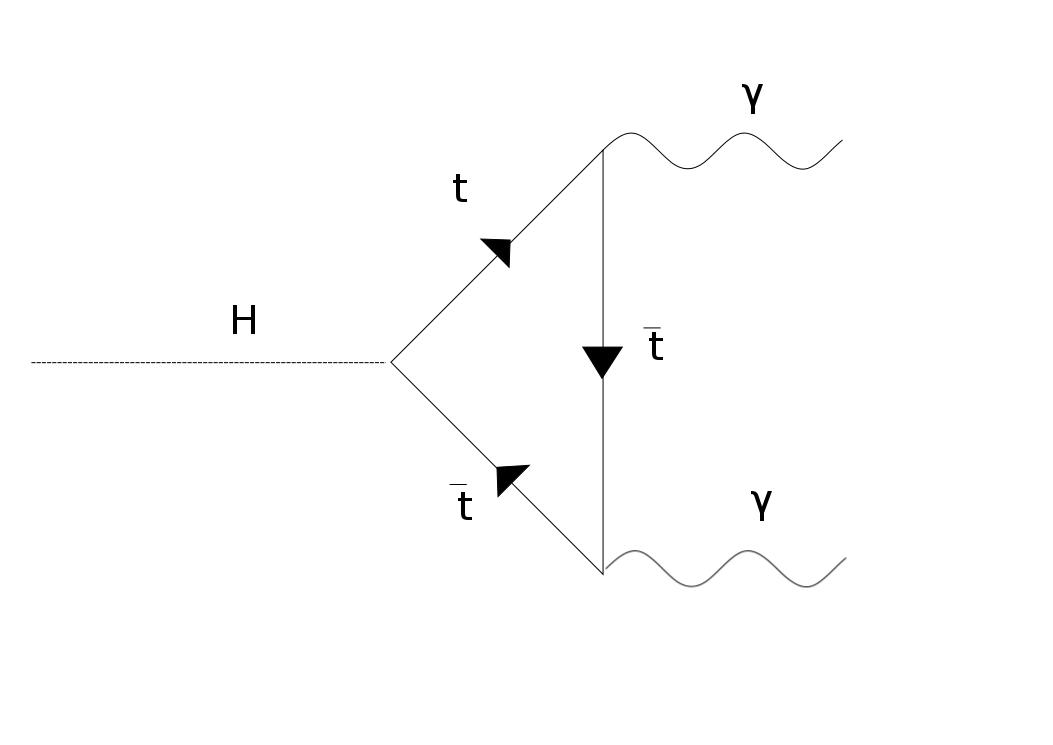
\includegraphics[scale=0.25]{higgsdecaydiphoton}
\section{Plan}
The photon data is simulated using 'Pythia' and outputs a series of 4 momenta (Energy and Momentum) of photons in a text file. The computational task is to take this text file, filter out all of the events into either Higgs produced photons (the Higgs signal) or background data.
\subsection{Programming}
The main programming language to do this is python. The main reason python is used was due to the more flexible nature of python compared to compiler based languages (such as C++) which would allow for changes to the program without rebuilding.
The disadvantage of this is that python files tend to be larger and less efficient for larger scale programs. Given that this project does not have large amounts of data to work with (the total size of the photon data file is around 300MB) python is not likely to run into such problems, however larger data files may require a complier based language to be used (such as C++).
\subsection{Filtering}
The 'signature' of the 2 photons produced by a Higgs decay that we are looking for has the following:
\begin{enumerate}
\item At least 2 photons per event
\item Transverse momentum $p_T > 20$ GeV for each photon
\item Energy $E > 20$ GeV
\end{enumerate}
This filtering often leaves 2 photon events that satisfy the criteria of being 2 Higgs events, however in the cases where more than 2 photons have the above properties, we employ 2 ways to 'pick' the photons produced by the Higgs.
\begin{enumerate}
\item Choose the 2 highest $p_T$ values for the photons
\item Find the 2 photons whose azimuthal angles $\phi$ between them is closest to $\pi$ rad.
\end{enumerate}
This then ensures all of the photon events selected will always be a diphoton system that satisfies the condition for being the result of a Higgs decay. 
The second method is more intensive in terms of operations to the data, but is more related to the Higgs decaying into 2 photons as opposed to assuming that the 2 largest $p_T$ are due to the Higgs. Again in the case where large data files are used it may be best to use the first method.
\subsection{Plotting the results}
The invariant masses of the diphoton systems in each event are calculated using
\begin{equation}
M_{\gamma \gamma}^2 = (E_{\gamma 1} + E_{\gamma 2})^2 - ({\bf p}_{\gamma 1} + {\bf p}_{\gamma 2})^2
\end{equation}
Since this is the invariant mass from a Higgs decay, this invariant mass (if a Higgs particle decayed into this system) should be present more often at $M_{\gamma \gamma} = M_{H}$. Where the (as of yet) best estimate for $M_{H} = 125.8$ GeV
\subsection{Weightings}
The Higgs signals (Higgs to diphoton) must be weighted by accounting for the probability that a Higgs is produced and that it decays into 2 photons. This is compared to the probability of getting a background signal of getting diphoton.
\begin{equation}
w = \frac{\sigma_{H} B_{H \rightarrow \gamma \gamma}}{\sigma_{\gamma \gamma}}
\end{equation}
Where $\sigma_{H}, \sigma_{\gamma \gamma}$ are the cross sections for producing Higgs and background photons respectively. The branching ratio of Higgs to 2 photons, $B_{H \rightarrow \gamma \gamma}$ is the ratio of the decay rate of Higgs to 2 photons to the total decay rate of the Higgs.
\section{Conclusion}
The project will use the following to look for a Higgs signal:
\begin{enumerate}
\item Parsing the data file of 4-momenta of photons
\item Filtering the photons that fit the profile of the Higgs decay
\item Calculate the invariant mass of the diphoton system
\item Plot the histogram of these invariant masses
\item Compare the peak (or lack of one) with the literature
\end{enumerate}
\end{document}
